\chapter{Evaluation}\label{chap:evaluation}

Neither persistent base nodes nor snapshotting lead to direct performance
benefits for Soup. Instead, they both come with a wide range of features and
improvements in other areas, further advancing Soup towards a production-ready
storage system. Moving the base node state to durable storage lets Soup operate
on datasets larger than its memory size, reduces its overall memory usage, and
improves the system's overall recovery capabilities---a necessity if Soup is
ever going to be usable for long running applications. Snapshotting takes this a
step further, and removes the performance penalty Soup sees while its partial
states are brought back to the state they were in prior to a fatal failure.

Regardless, Soup's performance when faced with a large amount of concurrent
requests is still one of its main contributions. While a certain reduction in
throughput and latency might be inevitable, it is crucial that this penalty
remains as insignificant as possible. This chapter first investigates the
effects \code{PersistentState} has on performance, followed by a look at the
recovery benefits from both \code{PersistentState} and snapshotting.

\newpage

\section{Write-performance}\label{sec:write-throughput}

Only a small subset of reads propagate all the way to the base nodes. Instead,
they are served by partially materialized nodes further down the graph, avoiding
the need for expensive computations on each read. This is not the case with
writes. Every update that reaches Soup needs to be fully persisted to durable
storage before a write acknowledgment can be sent. With persistent base nodes,
that involves materializing the updates into \code{PersistentState}. With
packets being processed synchronously at each domain, even the smallest increase
in write latency at the base nodes could have disastrous effects for the overall
write throughput of the system.

The \code{vote} benchmark described in section~\ref{sec:vote} is used to measure
write-performance. While it is normally a mixed-load benchmark, where clients
both write new votes and read the existing vote counts of articles, we will run
\code{vote} with a pure write-load, removing reads altogether. Since we are
measuring the impact of writing to durable storage, Soup will run without
sharding, resulting in a single domain writing new votes to
\code{PersistentState}. The database is prepopulated with 100K articles and the
inserted votes are uniformly distributed across the existing articles.

Soup can be run both in a local and distributed fashion, and \code{vote}
supports both. Writing to durable storage is a penalty fixed per machine
however, and benchmarking the horizontal scalability makes little sense.
Instead, we will use the \textit{local} \code{vote} benchmark, where both the
clients and the Soup workers run on the same machine.

The benchmark is run on the server described in section~\ref{sec:server-1}, with
the write-ahead log written to one SSD and the database files to another.

\begin{figure}[H]
  \includegraphics[width=\textwidth]{graphs/write-batch}
  \includegraphics[width=\textwidth]{graphs/write-sjrn}
  \caption{\
    Write-only comparison of Soup's regular write-ahead log and RocksDB.\@ The
    topmost figure shows the latency from when the request was initiated, while
    the bottommost includes the time from the request was generated by the
    open-loop benchmark (see section~\ref{sec:vote-open-loop}).
  }\label{fig:graph-write}
\end{figure}

Materializing base node state to durable storage introduces a slight
write-latency penalty under load. This eventually translates to about a 10\%
decrease in maximum write-throughput, compared to the naive Soup log. Even
though the RocksDB write-ahead log is written to a different disk than its
SS-tables, the amount of data that has to be written to the RocksDB WAL with
\code{PersistentState} is still multiples more than with the Soup log. The
former has to include entries for every index a base node maintains, while the
latter only needs one entry for the update itself.

Additionally, writing to RocksDB's in-memory buffers is not a negligible cost,
especially considering serialization. Whereas the Soup log only serializes
updates once, \code{PersistentState} needs to do so, in-part, once for each
index.

\subsection{MemTable format}

All writes to RocksDB are first placed in an in-memory buffer---a MemTable.
RocksDB includes multiple MemTable implementations, and the advantages and
disadvantages of the different data structures are described in
section~\ref{sec:memtable-impl}. To measure the impact of changing the MemTable
implementation, we make use of the \code{vote} benchmark from the previous
section, running on the same hardware.

\begin{figure}[H]
  \includegraphics[width=\textwidth]{graphs/memtable}
  \caption{\
    Write-latency measured at different throughput targets using the \code{vote}
    benchmark, while comparing separate RocksDB MemTable implementations.
  }\label{fig:graph-memtable}
\end{figure}

Changing from the default skip list implementation results in a significant
increase in write-throughput. In reality, this is a comparison of the $ O(\log
n) $ performance guarantees of a skip list and the closer to constant time
guarantees of the hash based implementations. RocksDB buckets keys based on the
their prefix, where the two hash based implementations use different data
structures to organize each bucket. Using a skip list for the buckets result in
$ O(\log p) $ insertions, where $ p $ is the amount of keys within a single
prefix. Linked list buckets improves this even further, with constant time
insertions and lower memory overhead.

While the write performance of the link list hash table is better than the skip
list one, its read performance is worse. The former requires a linear search to
find values, while the latter can do the same in logarithmic time. Fortunately,
RocksDB turns link list buckets into skip lists when they go beyond a certain
amount of keys---by default 256. In the \code{vote} benchmark this will likely
happen for the \code{Vote} base table, which will have a large index on
\code{article\_id}, but not for the \code{Article} table where each prefix maps
to a single key, a unique article.

\section{Read-performance}

When measuring the overall read-performance of Soup as a system, a read heavy
\code{vote} benchmark is a good indicator. To analyze the impact of durable
storage, we want to ensure that we are measuring the read performance of the
base nodes, and not the partial nodes further down the graph. Instead, we will
make use of the replay benchmark described in section~\ref{sec:bench-replay},
where each row is read at most once, resulting in a full replay from the base
nodes.

The database is prepopulated with 10 million rows, after which a small random
subset of the rows are read once. With \code{PersistentState}, Soup recovers
existing data between each test run, after flushing the disk caches.

The benchmark is run on the same server as the write-throughput benchmark (see
section~\ref{sec:server-1}).

\begin{figure}[H]
  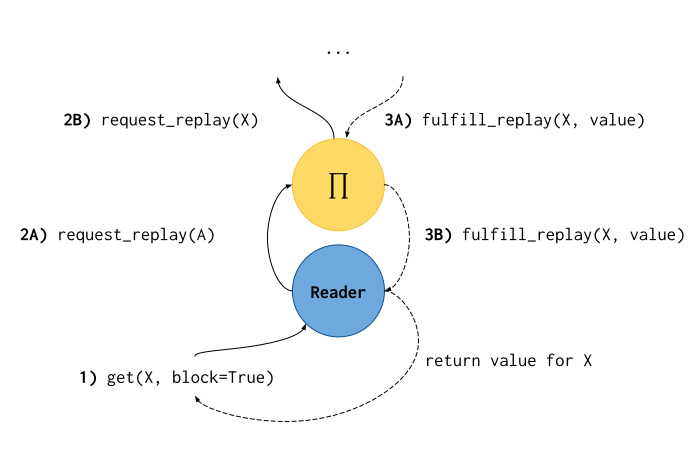
\includegraphics[width=\textwidth]{graphs/replay}
  \caption{\
    The replay performance of in-memory Soup compared to Soup with RocksDB.\@
  }\label{fig:graph-replay}
\end{figure}

Reading a small amount of rows result in less cache overlap when data is read
from durable storage, which in turn leads to higher read latency. When the
benchmark gravitates towards higher read counts, more data is bound to be served
from the file system cache, reducing the overall latency of most reads.

\subsection{SS-table format}

RocksDB provides two separate SS-table implementations, \code{BlockBasedTable}
and \code{PlainTable}, as described in section~\ref{sec:ss-table}. The latter
imposes limitations that the former does not have but promises lower read
latency on fast storage mediums in return.

\begin{figure}[H]
  \includegraphics[width=\textwidth]{graphs/replay-table}
  \caption{\
    Soup replay performance comparison between \code{BlockBasedTable} and
    \code{PlainTable}.
  }\label{fig:graph-replay-table}
\end{figure}

Soup's persistence base tables rely heavily on prefix iteration---one of
\code{PlainTable}'s design
goals\furl{rocksdb.org/blog/2014/06/23/plaintable-a-new-file-format.html}. This
results in significantly lower overall read latency compared to the traditional
block based format.

\section{Mixed workload}

The Lobsters benchmark described in section~\ref{sec:lobsters} is used to
measure the performance of persistent bases in a real-world setting. The
benchmark issues queries used in the real Lobsters web application, following a
distribution modeled after the application's production traffic. Whereas the
previous benchmarks measure queries per second, the Lobsters benchmark uses
pages per second as its metric, where separate pages require different queries.
A single page view can issue both read and write requests, through insertions,
lookups, and updates. As Soup translates updates to removals, followed by
insertions, the benchmark also measures deletion performance. The latency
measured is the \textit{sojourn} time of each request---the time from the
request is generated until completion (see section~\ref{sec:vote-open-loop}).

The benchmark runs on two separate servers. SQL queries are issued by a workload
generator and translated to native Soup requests using the MySQL shim layer (see
section~\ref{sec:mysql-shim}). These requests are handled by a separate server,
running Soup. Before initiating the benchmark, the database is prepopulated with
a similar amount of data to the real Lobsters application: 120,000 comments,
40,000 stories, and 9,200 users. Afterwards, the benchmark issues requests
following a target throughput goal.

Note that unlike the write-throughput benchmark, Soup's write-ahead log is not
used here. Instead, the benchmark compares purely in-memory---and not
durable---Soup, to Soup with its base tables safely stored in durable RocksDB.\@

\subsection{Computational overhead}

The Lobsters benchmark is run on two separate hardware configurations. The
first, server setup 2 (described in section~\ref{sec:server-2}), emulates
durable storage using a
RAM-disk\furl{https://manpages.debian.org/stretch/initscripts/tmpfs.5.en.html}.
This lets the benchmark focus on the computational overhead of storing Soup's
base tables in RocksDB, while serving as a useful comparison to existing Soup
benchmarks---which make use of the same server setup.

\begin{figure}[H]
  \includegraphics[width=\textwidth]{graphs/lobsters-ram}
  \caption{\
    The 99th percentile sojourn latency of the Lobsters benchmark measured at
    increasing throughput. The \code{soup} target does not write any log files,
    while the \code{rocksdb\_soup} target persists all updates to RocksDB.
  }\label{fig:lobsters-ram}
\end{figure}

Figure~\ref{fig:lobsters-ram} shows that Soup with its base tables stored in
RocksDB performs just as well as in-memory Soup. The seemingly random
fluctuations in latency exist for both versions, and are not a result of whether
the tables are stored in-memory or not.

\subsection{I/O overhead}

To measure the overhead of having to persist updates to a durable
write-ahead log, the same benchmark is run on an Amazon EC2 server with an NVMe
SSD-drive\furl{https://docs.aws.amazon.com/AWSEC2/latest/UserGuide/ssd-instance-store.html}
(server setup 2 in section~\ref{sec:server-2}). Similar to the write-throughput
benchmark in section~\ref{sec:write-throughput}, the write-ahead log and RocksDB
database files are written to separate disks.

\begin{figure}[H]
  \includegraphics[width=\textwidth]{graphs/lobsters-nvme}
  \caption{\
    99th percentile sojourn latency of the Lobsters benchmark measured at
    increasing throughput. The \code{rocksdb\_soup} target writes to a durable
    NVMe SSD.\@
  }\label{fig:lobsters-nvme}
\end{figure}

The observed latency is slightly higher when Soup's base tables are stored on
durable storage, but the difference is far from significant. The server used
here is on the other hand far slower than the one in the previous section,
resulting in overall lower throughput targets. While durable and non-durable
Soup are quite equal here as well, the difference would without doubt be more
drastic on a server with slower storage media.

\section{Recovery}

The recovery benchmark introduced in section~\ref{sec:bench-recovery} helps us
compare the recovery impact imposed by different durability strategies. For
every data point, the database is populated with 10K articles and a varying
amount of votes divided evenly between the articles. After population, Soup is
restarted, while the time it takes to recover is measured. The state is
considered recovered when the total sum of votes returned from reading all
articles equal the actual amount of votes in the system---signified as
\textit{total} in figure~\ref{fig:graph-recovery}.

Unlike the other durability methods, recovering with durable base nodes does not
affect the partial nodes further down the graph---they remain empty until future
read operations trigger ancestor queries to the base nodes. Snapshotting, on the
other hand, brings all materialized nodes in the graph back to the state they
were in prior to crashing. This is the case for log-recovery as well, as updates
from the WAL propagate through the entire graph when recovering. To highlight
this divide, the time it takes to read a single key after recovering from a
durable base node application is measured as well, denoted as \textit{initial}
in figure~\ref{fig:graph-recovery}.

\begin{figure}[H]
  \includegraphics[width=\textwidth]{graphs/recovery}
  \caption{\
    The recovery benchmark measures the time it takes to recover after
    a failure. The \textit{initial} metric highlights the latency of reading a
    single key, while \textit{total} requires all reads to return the same
    result as prior to crashing.
  }\label{fig:graph-recovery}
\end{figure}

The results are pretty much as expected. Snapshotting returns all the
materialized nodes in the graph to their correct state, avoiding the need to
replay any state after recovering. The time it takes to recover still increases
after a while, with more data to read from disk. Log-based recovery needs to go
through \textit{all} updates since the beginning of time before it is considered
ready, resulting in poor performance. With durable base nodes, each read
requires a full replay from the bases---a significant latency penalty when the
row count goes up.

With \code{PersistentState}, the base nodes do not have to process any updates
at all when recovering. Restoring \code{PersistentState} to the correct state is
left to RocksDB, which puts a cap on recovery time by ensuring that its
write-ahead logs never grow beyond a given size. Recovering the actual database
files, the SS-tables, is ``free''---no data needs to be read into memory.

\subsection{Snapshot compression}

Compressing snapshots introduce a trade-off between computation and storage
overhead. Depending on the underlying hardware, the penalty induced from having
to compress and decompress snapshots might be amortized by the reduced I/O
usage. To measure the impact on recovery performance, the benchmark used in the
previous section is run on the same hardware---with and without \code{zlib}
compression.

\begin{figure}[H]
  \includegraphics[width=\textwidth]{graphs/snapshot-compressed}
  \caption{\
    The total snapshot recovery time, with and without compression.
  }\label{fig:snapshot-compressed}
\end{figure}

Recovering from compressed snapshots takes on average three times as long as
recovering from regular snapshots. This is measured on a server with a
SSD-drive, and the gap would without doubt be less significant on slower storage
media. Regardless, with a focus on reducing recovery time, this is not a
trade-off we are willing to make.

\subsection{Write-performance with snapshotting}\label{sec:snapshot-write}

Snapshotting is a significant improvement to Soup's recovery situation and a
step in the right direction for Soup as a production-ready system. Regardless,
it is only useful if Soup manages to maintain much of the same write-throughput
while performing regular snapshots.

To measure the performance penalty of snapshotting, we make use of the
\code{vote} benchmark described in section~\ref{sec:vote} and earlier in this
chapter. The benchmark compares the batch write latency at increasing throughput
targets, both with and without snapshotting. The benchmark runs for 60 seconds,
performing a snapshot every 10 seconds.

\begin{figure}[H]
  \includegraphics[width=\textwidth]{graphs/write-snapshot-batch}
  \caption{\
    Write-latency comparison with and without snapshotting (with a snapshot
    timeout of 10 seconds). Both use Soup's regular write-ahead log.
  }\label{fig:graph-snapshot}
\end{figure}

Most of the snapshotting work is performed in standalone snapshot workers,
running in threads separate from Soup's packet processing. Without this, the
throughput penalty would without doubt be much more significant than the 10\%
observed in figure~\ref{fig:graph-snapshot}. The penalty is a result of the full
state clone incurred at each materialized node during a snapshot.

\begin{figure}[H]
  \includegraphics[width=\textwidth]{graphs/write-snapshot-100-batch}
  \caption{\
    100th percentile comparison, with and without snapshotting.
  }\label{fig:graph-snapshot-100}
\end{figure}

The first snapshot graph shows no increase in latency. With a snapshot timeout
of 10 seconds and a benchmark runtime of 60 seconds, snapshot occurrences are
probably too rare for it to show up in the 95th percentile. Looking at the 100th
percentile on the other hand, we can see the latency spiking at a lower
throughput than normal. At this point the state size is reasonably large,
resulting in non-trivial clone operations.
